\documentclass{article}

% Packages
\usepackage[utf8]{inputenc} % For modern characters
\usepackage{microtype} % For sexy kerning
\usepackage{mathtools} % For math stuff
\usepackage{amssymb} % For math symbols
\usepackage{tabularx} % For making tables
\usepackage{fancyhdr} % Use a header
\usepackage{pdfpages} % For including a graphics path

% Set the margins
\usepackage[scale=0.8, top=1in, bottom=1in]{geometry}

% Other front matter
\graphicspath{ {img/} } % Put all images in img/
\newcommand{\code}[1]{\texttt{#1}} % More readable for writing inline code.
\newcommand{\p}[1]{\paragraph{#1}} % Easier to type out for paragraph command
\newcommand{\addsection}[1]{\addcontentsline{toc}{section}{#1}} % content lines
\newcommand{\addsubsection}[1]{\addcontentsline{toc}{subsection}{#1}} % content lines
\pagestyle{fancy} % Makes Header Possible
{ %%% Header Set up
	\lhead{} % Set the left header to be blank
	\chead{} % Set the center header to be blank
	% Header for every page except the first two
	\rhead{Ben Foster | Homework 5 | May 14, 2015} % Name, assignment, date
}
\setcounter{tocdepth}{2} % Set Table of Contents Depth
\setlength{\parindent}{0pt} % Disable automatic indentation

%%%%%%%%%%%%%%%%%%%%% Begin Document %%%%%%%%%%%%%%%%%%%%%
\begin{document}

{ % Title page, table of contents, and page number setting
	\title{Probability and Statistics for Engineers Homework Five \\ TMATH 390}
	\author{Ben Foster\thanks{
		Institute of Technology, University of Washington Tacoma} \\
		Instructor: Julia Eaton}
	\date{May 14, 2015} % Include the date
	\maketitle % Make the title
	\thispagestyle{empty} % No page number at bottom
	\clearpage % Start the table of contents on the next page
	
	\pagenumbering{roman} % Use roman numerals for numbering
	\tableofcontents % Make the table of contents
	\clearpage % Start homework on next page
	\setcounter{page}{1} % Begin numbering over again
	\pagenumbering{arabic} % use arabic numerals for numbering
}

\section*{Problem 1} %%% DONE
\addsection{First Problem}

	A college library has five copies of a certain text on reserve. Two copies (1 and 2) are first 
	editions, and the other three (3, 4, and 5) are second editions. A student examines these books in 
	random order, stopping only when a second edition has been selected. One outcome is 4, and 
	another is 215. \\

	(a) List all outcomes in the sample space $S$. \\
	(b) Let $A$ denote the event that exactly one book must be examined. What outcomes are in $A
	$? \\
	(c) Let $B$ be the event that book 4 is the one selected. What outcomes are in $B$? \\
	(d) Let $C$ be the event that book 2 is not examined. What outcomes are in $C$? \\

	\addsubsection{Answer to 1.a}
	\p{Answer to a} The sample space of an experiment are all of the possible outcomes of a chance 
	experiment. The sample space for this chance experiment is:
	\[ S = [3,4,5,13,14,15,23,24,25,123,124,125,213,214,215] \]
	
	\addsubsection{Answer to 1.b}
	\p{Answer to b} The event that exactly one book must be examined means that the student 
	randomly picked up a second edition book first:
	\[ A = [3,4,5] \]
	
	\addsubsection{Answer to 1.c}
	\p{Answer to c} The event that book 4 is selected doesn't necessarily mean that it is the first book 
	selected, but it could also be the second or third after one or both of the first two first edition 
	books were selected:
	\[ B = [4,14,25,124,214] \]
	
	\addsubsection{Answer to 1.d}
	\p{Answer to d} The event that book 2 is not examined means that we could have any simple 
	event that does not contain 2:
	\[ C = [3,4,5,13,14,15] \]

\clearpage
\section*{Problem 2} %%% DONE
\addsection{Second Problem}

	An engineering firm is constructing power plants at three different sites. \\
	Define the events $E_1$, $E_2$, and $E_3$ as follows:
	\begin{itemize}
		\item{$E_1 =$ the plant at site 1 is completed by the contract date.}
		\item{$E_2 =$ the plant at site 2 is completed by the contract date.}
		\item{$E_3 =$ the plant at site 3 is completed by the contract date.}
	\end{itemize}
	Draw a Venn diagram that depicts these three events as intersecting circles. Shade the region on 
	the Venn diagram corresponding to each of the following events (redraw the Venn diagram for 
	each question): \\
	
	(a) At least one plant is completed by the contract date. \\
	(b) All plants are completed by the contract date. \\
	(c) None of the plants are completed by the contract date. \\
	(d) Only the plant at site 1 is completed by the contract date. \\
	(e) Exactly one of the three plants is completed by the contract date. \\
	(f) Either the plant at site 1 or site 2 or both of the two plants are completed by the contract date.\\
	
	Original Venn diagram:
	\begin{center}
		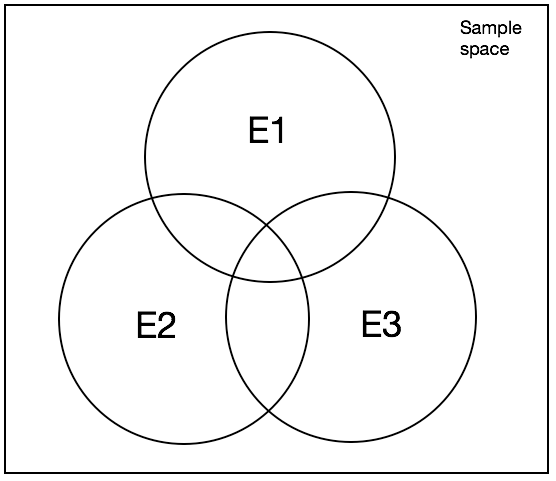
\includegraphics[width=5in]{prob2_orig.jpg}
	\end{center}
	
	\clearpage
	\addsubsection{Answer to 2.a}
	\p{Answer to part a}
	\begin{center}
		\includegraphics[width=4.5in]{prob2_a.jpg}
	\end{center}
	
	\addsubsection{Answer to 2.b}
	\p{Answer to part b}
	\begin{center}
		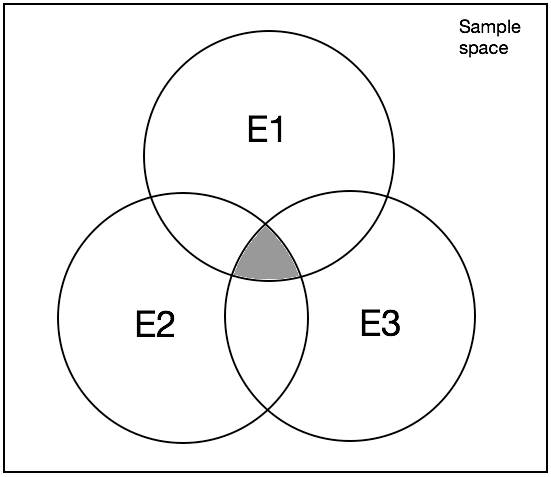
\includegraphics[width=4.5in]{prob2_b.jpg}
	\end{center}
	
	\clearpage
	\addsubsection{Answer to 2.c}
	\p{Answer to part c}
	\begin{center}
		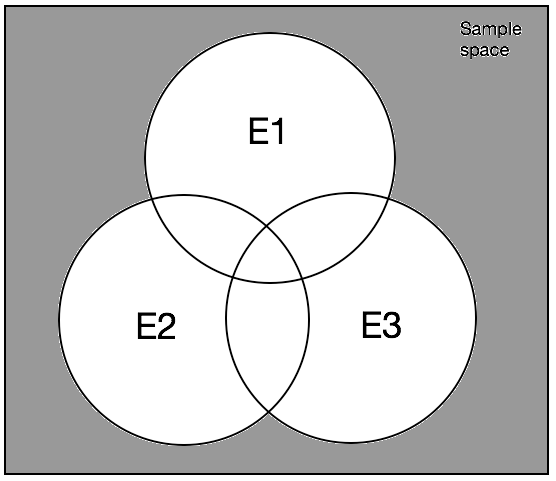
\includegraphics[width=4.5in]{prob2_c.jpg}
	\end{center}
	
	\addsubsection{Answer to 2.d}
	\p{Answer to part d}
	\begin{center}
		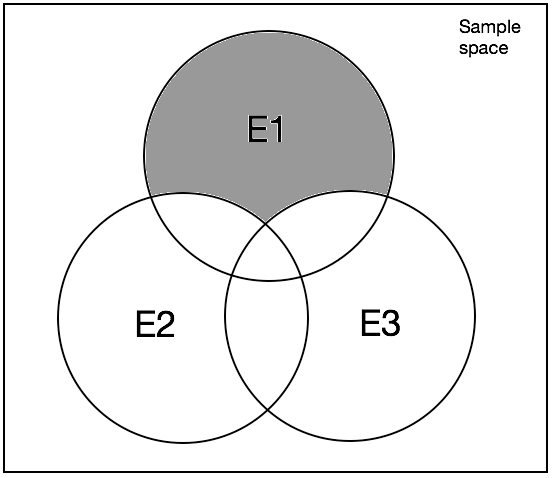
\includegraphics[width=4.5in]{prob2_d.jpg}
	\end{center}
	
	\clearpage
	\addsubsection{Answer to 2.e}
	\p{Answer to part e}
	\begin{center}
		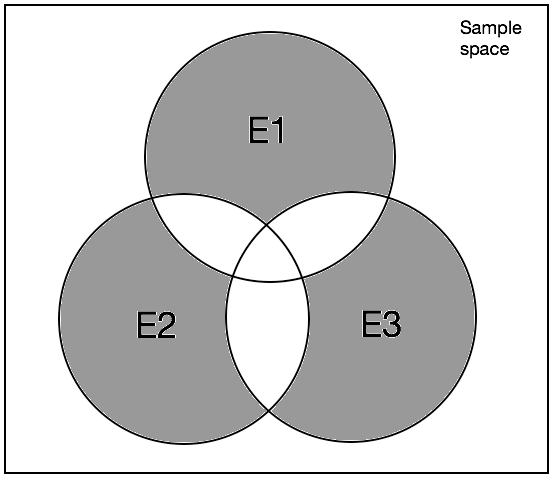
\includegraphics[width=4.5in]{prob2_e.jpg}
	\end{center}
	
	\addsubsection{Answer to 2.f}
	\p{Answer to part f}
	\begin{center}
		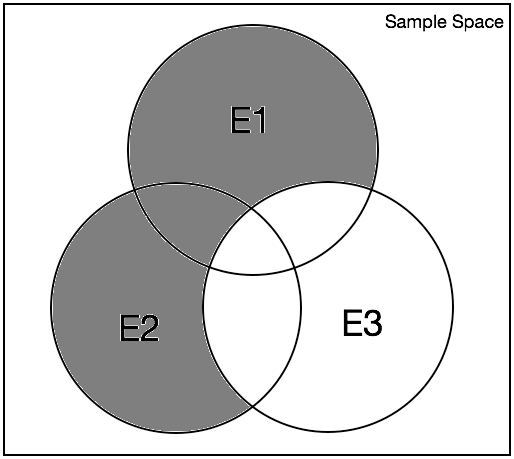
\includegraphics[width=4.5in]{prob2_f.jpg}
	\end{center}
	
\clearpage	
\section*{Problem 3} %%% DONE
\addsection{Third Problem}

	Let $A_i = i\text{th}$ student got a perfect score on midterm 1, for $i = 1,...,18$. \\

	
	(a) Interpret $\left( \overset{18}{\underset{i=1}{\cap}} A_i \right)^\prime$ in English. \\
	(b) Interpret $\overset{18}{\underset{i=1}{\cup}} A_i^{\prime}$ in English. Is it equivalent to part a?
	
	\addsubsection{Answer to 3.a}
	\p{Answer to a}
	$\left( \overset{18}{\underset{i=1}{\cap}} A_i \right)^\prime$ is the same as saying the 
	complement of $A_1$, and $A_2$, and ... and $A_18$. Basically, students 1 through 18 did not 
	get a perfect score on the first midterm, but any other combination of these students getting a 
	perfect score on the first midterm is possible (i.e. $A_1$ and $A_2$).
	
	\addsubsection{Answer to 3.b}
	\p{Answer to b}
	$\overset{18}{\underset{i=1}{\cup}} A_i^{\prime}$ is the same as saying $A_1^\prime$, or
	$A_2^\prime$, or ... or $A_{18}^\prime$. Basically, any combination of students 1 through 18 
	can get a perfect score on their first midterm, however it is not possible for all 18 students to get a 
	perfect score. \\
	
	Part a and part b are the same.

\section*{Problem 4} %%% DONE
\addsection{Fourth Problem}

	Using everything we have learned about events and probability, prove that
	\[ P(A|B) + P(A^{\prime}|B) = 1 \]
	Do not assume that events $A$ and $B$ are independent (i.e. $P(A\cap B) \not= P(A)\cdot P(B)
	$). Explain each step of your calculation.
	
	\addsubsection{Answer to 4}
	\p{Answer to problem 4}
	$P(A|B) =$ the conditional probability of A occurring given that event B has already occurred. We 
	know that these probabilities must be between 0 and 1, so $0 \le P(A|B) \le 1$ and $ 0 \le 
	P(A^{\prime}|B) \le 1$. Also, from the definition, we know that event $B$ has already occurred, so 
	we're really just adding together the probabilities of wether $A$ will occur or not. $P(A|B)$ is the 
	probability that A will occur and $P(A^{\prime}|B)$ is the probability that $A$ will not occur. Since 
	there are only two possibilities, then the summation of those two possibilities should equal 1, or a 
	100\% chance. Meaning that there is a 100\% chance that $A$ will either occur or not occur given 
	that $B$ has already occurred.

\clearpage	
\section*{Problem 5} %%% DONE
\addsection{Fifth Problem}

	Five companies (A, B, C, D, and E) that make electrical relays compete each year to be the sole 
	supplier of relays to a major automobile manufacturer. The auto company's records show that the 
	probabilities of choosing a company to be the sole supplier are
	\begin{center}
	\begin{tabular}{ l r r r r r }
		Supplier chose: & A & B & C & D & E \\
		Probability: & 0.30 & 0.20 & 0.10 & 0.25 & 0.15
	\end{tabular}
	\end{center} 
	
	(a) Suppose that supplier E goes out of business this year, leaving the remaining 4 companies to 
	compete with one another. What are the new probabilities of companies A, B, C, and D being 
	chosen ad the sole supplier this year? \\
	(b) Suppose the auto company narrows the choice of suppliers to companies A and C. What is 
	the probability that company A is chosen this year?
	
	\addsubsection{Answer to 5.a}
	\p{Answer to a}
	If company E were to go out of business then to determine the probabilities of the other 
	companies being chosen, we have to use the equation:
	\[ P(\text{Other Company} | E^{\prime}) \]
	\[ = \frac{P(\text{Other Company})}{P(E^{\prime})} \]
	This gives us a new table:
	\begin{center}
	\begin{tabular}{ c c c c }
		A & B & C & D \\
		0.3529 & 0.2352 & 0.1176 & 0.2941
	\end{tabular}
	\end{center}
	
	\addsubsection{Answer to 5.b}
	\p{Answer to b}
	If we narrowed down our decision to companies A and C, then we would use the equations:
	\[ P(A|B^\prime + D^\prime + E^\prime) = \frac{P(A)}{P(B^\prime + D^\prime + E^\prime)} \]
	\[ = \frac{0.3}{1 - (0.2+0.25+0.15)} \]
	\[ = 0.75 \]
	and
	\[ P(C|B^\prime + D^\prime + E^\prime) = \frac{P(C)}{P(B^\prime + D^\prime + E^\prime)} \]
	\[ = \frac{0.1}{1 - (0.2+0.25+0.15)} \]
	\[ = 0.25 \]
	Therefore there is a 75\% chance of choosing company A and a 25\% chance of choosing 
	company C.

\clearpage
\section*{Problem 6} %%% DONE
\addsection{Sixth Problem}

	Number 5.16 in your book on page 214: \\
	In Exercise 6, suppose that there is a probability of 0.01 that a digit is incorrectly sent over a 
	communication channel (i.e., that a digit sent as a 1 is received as a 0, or vice versa). Consider a 
	message that consists of exactly 60\% 1s. \\
	
	(a) What is the proportion of 1s received at the end of the channel? \\
	(b) If a 1 is received, what is the probability that a 1 was sent? Hint: Use the tree diagram from 
	Exercise 6. \\
	
	\addsubsection{Answer to 6.a}
	\p{Answer to a}
	Since our original message consists of 60\% 1s and since those 1s have a 99\% chance of 
	staying a 1 (1 - 0.01 from the probability that they will change) and since we also have 40\% 0s in 
	the original message and they have a 1\% chance of turning into 1s then we can use this 
	calculation to determine the proportion of 1s in the final message:
	\[ (0.6 \times 0.99) + (0.4 \times 0.01) = 0.598 \]
	So 59.8\% of the received message will be comprised of 1s.
	
	\addsubsection{Answer to 6.b}
	\p{Answer to b}
	If a 1 is received then there is a 99\% chance that a 1 was sent since there is a 1\% chance of an 
	error. We also know that the message being sent consists of 60\% 1s. Therefore we use the 
	formula:
	\[ P(S|R) = \frac{P(S\text{ and }R)}{P(R)} \]
	\[ = \frac{0.99(0.6)}{0.598} \]
	\[ = 0.993311 \]
	So we have a 99.33\% chance that the sent bit will be a 1 if we receive a 1.

\clearpage	
\section*{Problem 7} %%% DONE
\addsection{Seventh Problem}

	Number 5.19 in your book on page 214: \\
	In forensic science, the probability that any two people match with respect to a given 
	characteristic (hair color, blood type, etc.) is called the \textit{probability of a match}. Suppose that 
	the frequencies of blood phenotypes in the population are as follows: \\
	\begin{tabular}{ c c c c }
		A & B & AB & O \\
		0.42 & 0.10 & 0.04 & 0.44
	\end{tabular} \\
	
	(a) What is the probability that two randomly chosen people both have blood type A? \\
	(b) Repeat the calculation in part (a) for the other three blood types. \\
	(c) Find the probability that two randomly chosen people have matching blood types. Note: A 
	person can have only one phenotype. \\
	(d) The probability that two people do not match for a given characteristic is called 
	\textit{discriminating power}. What is the discriminating power for the comparison of two people's 
	blood types in part (c)?
	
	\addsubsection{Answer to 7.a}
	\p{Answer to a}
	Since we have a 42\% chance of randomly picking a person with blood type A, then randomly 
	picking two people with this blood type would be $0.42 \times 0.42 = 0.1764$. We have a 17.6\% 
	chance of randomly choosing two people with blood type A.
	
	\addsubsection{Answer to 7.b}
	\p{Answer to b}
	Repeating the same calculation in part A, we get: \\
	$0.10 \times 0.10 = 0.01$ \\
	$0.04 \times 0.04 = 0.0016$ \\
	$0.44 \times 0.44 = 0.1936$ \\
	So we have a 1\% chance of choosing two people with blood type B, a 0.2\% chance of choosing 
	two people with blood type AB, and a 19.4\% chance of choosing two people with blood type O.
	
	\addsubsection{Answer to 7.c}
	\p{Answer to c}
	To find this probability, all we have to do is sum together the probabilities found in part a and b:
	\[ 0.01 + 0.0016 + 0.1936 + 0.1764 = 0.3816 \]
	We have a 38.2\% chance of choosing two people that have the same blood type.
	
	\addsubsection{Answer to 7.d}
	\p{Answer to d}
	The probability that two people do not match blood types is basically the opposite of the previous 
	question so $1-0.3816 = 0.6184$. We have a 61.8\% chance of choosing two people who don't 
	have a matching blood type.

\clearpage	
\section*{Problem 8} %%% DONE
\addsection{Eighth Problem}

	Number 5.21 in your book on page 214: \\
	Consider a system of components connected as shown in the following figure: \\
	\begin{center}
		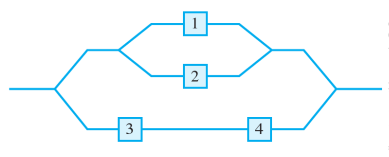
\includegraphics[width=4in]{prob8.jpg}
	\end{center}
	Components 1 and 2 are connected in parallel, so that their subsystem functions correctly if 
	either component 1 or 2 functions. Components 3 and 4 are connected in series, so their 
	subsystem works only if both components work correctly. \\
	
	If all components work independently of one another and P(a given component works) = 0.9, 
	calculate the probability that the entire system works correctly.
	
	\addsubsection{Answer to 8}
	\p{Answer to problem 8}
	To solve this problem we need to find the probability $P((1\text{ or }2)\text{ or }(3\text{ and }4))$ 
	with $P(1) = P(2) = P(3) = P(4) = 0.9$.
	\[ P(1\text{ or }2) = 1 - P(1')P(2') = 1-0.01 = 0.99 \]
	\[ P(3\text{ and }4) = P(3)P(4) = (0.9)(0.9) = 0.81 \]
	Now we can treat the top and bottom parts of the system as single events A and B respectively 
	where $P(A) = 0.99$ and $P(B) = 0.81$.
	\[ P(A\text{ or }B) = P(A) + P(B) - P(A\text{ and }B) \]
	\[ = 0.99 + 0.81 - 0.8019 \]
	\[ = 0.9981 \]
	So there is a 99.81\% chance that the entire system works correctly.
	

\clearpage	
\section*{Problem 9} %%% DONE
\addsection{Ninth Problem}

	Let $p$ be the sample proportion, written as $p = \frac{n_f}{n}$, where $n =$ sample size, and 
	$n_f =$ the number of females in the sample. Show that $E[p] = \pi$ and $V[p] = \frac{\pi(1-\pi)}
	{n}$, where $\pi =$ proportion of females in population. Hint: Use what you know about Binomial 
	distributions.
	
	\addsubsection{Answer to 9}
	\p{Answer to problem 9} Recall that for the binomial distribution:
	\[ E[X] = n\pi \]
	\[ V[X] = n\pi(1-\pi)  = E[X^2] - (E[X])^2 \]
	so
	\[ E[p] = E[\frac{n_f}{n}] \]
	Since n is a constant
	\[ = \frac{1}{n}E[n_f] = \frac{n\pi}{n} = \pi \]
	and
	\[ V[p] = V[\frac{n_f}{n}] \]
	Since n is a constant
	\[ = \frac{1}{n^2}V[n_f] = \frac{n\pi(1-\pi)}{n^2} = \frac{\pi(1-\pi)}{n} \]

\section*{Problem 10} %%% DONE
\addsection{Tenth Problem}

	A survey of the members of a large professional engineering society is conducted to determine 
	their views on proposed changes to an ASTM measurement standard. Suppose that 80\% of the 
	entire membership favor the proposed changes. Hint: Use the result from the previous problem. \\
	
	(a) Calculate the mean and standard deviation of the sampling distribution of the proportion of 
	engineers in samples of size 25 who favor the proposed changes. \\
	(b) Calculate the mean and standard deviation of the sampling distribution of the proportion of 
	engineers in samples of size 100 who favor the proposed changes.

	\addsubsection{Answer to 10.a}
	\p{Answer to a}
	Using the idea that $E[p] = \pi$ and $V[p] = \frac{\pi(1-\pi)}{n}$:
	\[ E[p] = \pi = 0.8 \]
	\[ \sigma = \sqrt{V[p]} = \sqrt{\frac{0.8(1-0.8)}{25}} \]
	\[ \sigma = 0.08 \]
	
	\addsubsection{Answer to 10.b}
	\p{Answer to b}
	Using the idea that $E[p] = \pi$ and $V[p] = \frac{\pi(1-\pi)}{n}$:
	\[ E[p] = \pi = 0.8 \]
	\[ \sigma = \sqrt{V[p]} = \sqrt{\frac{0.8(1-0.8)}{100}} \]
	\[ \sigma = 0.04 \]

\clearpage	
\section*{Problem 11} %%% DONE
\addsection{Eleventh Problem}

	The lifetime of a certain battery is normally distributed with a mean value of 8 hours and a 
	standard deviation of 1 hour. There are four such batteries in a package. \\
	
	(a) What is the probability that the average lifetime of the four batteries exceeds 9 hours? \\
	(b) If $T$ denotes the average lifetime of the four batteries in a randomly selected package, find 
	the numerical value of $T_0$ for which $P(T \ge T_0) = 0.95$.
	
	\addsubsection{Answer to 11.a}
	\p{Answer to a}
	In order to solve this, we need to find $P(x > 9)$. In this case, since we know that the lifetime of 
	the battery is normally distributed, then we can use the standard normal table to help us find our 
	answer. Now we use $P(z > \frac{9-\mu_{\bar{x}}}{\sigma_{\bar{x}}})$ where $\mu_{\bar{x}} = 8$ 
	and $\sigma_{\bar{x}} = \frac{\sigma}{\sqrt{n}} = \frac{1}{2}$. From this, $P(z > 2) = 1-P(z<2)$. 
	Using the table, we get  0.0228 for the proportion of time that the lifetime exceeds 9 hours. We 
	could also say that we have a 2.28\% chance that the average lifetime of the four batteries will 
	exceed 9 hours.
	
	\addsubsection{Answer to 11.b}
	\p{Answer to b}
	For this problem, we know that $P(T \ge T_0) = 0.95$. From this, we know that $P(T \ge T_0) = 1 
	- P(T < T_0)$ so $P(T<T_0) = 0.05$. Now we just do a reverse table look up and we get the 
	following:
	\[ -1.645 = \frac{T_0 - 8}{0.5} \]
	\[ T_0 = 7.1775 \]

\clearpage	
\section*{Problem 12} %%% DONE
\addsection{Twelfth Problem}

	The number of flaws $x$ on an electroplated automobile grill is known to have the following 
	probability mass functions: $p(0) = 0.6$, $p(1) = 0.2$, $p(2) = 0.1$, $p(3) = 0.1$. \\
	
	(a) Calculate the mean and standard deviation of $x$. \\
	(b) What are the mean and standard deviation of the sampling distribution of the average number 
	of flaws per grill in a random sample of 50 grills? \\
	(c) For a random sample of 50 grills, calculate the approximate probability that the average 
	number of flaws per grill exceeds 0.8.
	
	\addsubsection{Answer to 12.a}
	\p{Answer to a}
	For the mean:
	\[ \mu = \sum xp(x) \]
	\[ = 0(0.6) + 1(0.2) + 2(0.1) + 3(0.1) \]
	\[ = 0.7 \]
	For the standard deviation
	\[ \sigma = \sqrt{\sum(x-\mu)^2p(x)} \]
	\[ = \sqrt{((0-0.7)^20.6) + ((1-0.7)^20.2) + ((2-0.7)^20.1) + ((3-0.7)^20.1)} \]
	\[ = \sqrt{0.294 + 0.018 + 0.169 + 0.529} \]
	\[ = \sqrt{1.01} \]
	\[ = 1.01 \]
	
	\addsubsection{Answer to 12.b}
	\p{Answer to b}
	For the mean:
	\[ \mu_{\bar{x}} = \mu = 0.7 \]
	For the standard deviation:
	\[ \sigma_{\bar{x}} = \frac{\sigma}{\sqrt{n}} \]
	\[ = \frac{1.01}{\sqrt{50}} \]
	\[ = 0.1421 \]
	
	\addsubsection{Answer to 12.c}
	\p{Answer to c}
	We need to find $P(x>0.8)$ which is the same as saying $P(z > \frac{0.8-\mu}{\sigma}$ since we 
	are looking at a normal distribution. From this we get $P(z > 0.70359)$. Now we just have to look 
	at the standard normal table. Since we want something greater than a number, then we can just 
	do $1-P(z<0.704)$ to get the same thing. From looking at the table, we get
	\[ P(z > 0.704) = 1 - 0.7580 \]
	\[ P(z > 0.704) = 0.242 \]

\end{document}
